\documentclass[12pt]{thesis}
\usepackage[utf8]{inputenc}
\usepackage[english]{babel}
\usepackage{graphicx}


\begin{document}

\title{Smoothed Particles Hydrodynamics for Impact Simmulation}
\author{J. Camilo Alfonso R.}
\date{\today}
\maketitle

\tableofcontents

\part{Bibliograpfic Revision}

\chapter{Liu \& Liu}

\section{Introduction}
In the SPH method, the state of a system is represented by a set of particles, which possess individual material properties and move according to the governing conservations equations.\\
The principal characteristics of the SPH method are:
\begin{itemize}
\item Adaptive Nature: Any domain can be described by an arbitrary set of particles. The Sph Approximation does not get effected by the particle distribution.
\item Meshfree: SPH does not uses a any mesh to provide interactions between particles. The field values are evaluated for all particles at each time step, which makes SPH esay to track the properties of particles in time. This property tracking is specially difficult for othr numerical methods that use Eulerian mesh.
\end{itemize} 
SPH simmulation involves two major steps: particle representation and particle approximation. The particle representation is related to only the initial creation fo the particles.
Sph is important because:
\begin{itemize}
\item SPH have recently reached an acceptable level for practical engineering applications
\item Applicable in CFD, CSM, from micro-scale to macro-scale and astronomical-scale, fromd discrete to continuum systems.
\item SPH have been introduced in commercial codes \cite{Liu_SPH}
\end{itemize}

\section{SPH Concept and Essential Formulation}
The general solution procedure of SPH is:
\begin{enumerate}
\item The problem domain is represented by a set of arbitrarily distribuited particles. NO connectivity of these particles is needed \textit{(Meshfree)}
\item The \textit{integral representation method} is used for field function representation. \textit{Kernel approxiamtion}. \textit{(Integral function representation)}
\item The kernel approximation is the further approxiamted using particles (\textit{Particle Approxiamtion}). It is done by replacing the integration in the integral representation of the field functions and its derivates with summations over all the corresponding values at the neighboring in a local domain called \textit{Support domain}. \textit{(Compact Support)}
\item The particle approxiamtion is performed at every tinme step, and hence the use of the particle depends on the current local distribution of the particles. \textit{Adaptive)}
\item The particle approxiamtions are performed to all the terms related to the fields function in the PDEs to produce a set of ODEs in discretized form with respecto to time only. \textit{(Langrangian)}
\item The ODEs are solved using an \textit{explicit} integration algorithm to achieve fast time stepping, and to obtain the time history of all the field variables for all the particles. \textit{Dynamic}
\end{enumerate}
The combination of the 6-point strategy makes the SPH method be a meshfree, adaptive, stable and Lagrangian solver for Dynamic problems.

\subsection{Essential Formulation of SPH}
\textbf{Integral Representation of a function and derivative}\\
A function can be represented in an integral form (Eq. 2.1 in \cite{Liu_SPH}):
\[f(x)=\int_{\Omega}{f(x\prime)W(x-x',h)dx'}\]
\begin{itemize}
\item $f$ is a function of the tree-dimensional postion vector x
\item $W(x-x',h)$ Smoothing function (\textit{kernel}), $h$ is the \textit{smoothing length} definig the influence area of the smoothing function.
\end{itemize}
The derivative of a function also can be approximated as (Eq. 2.15 in \cite{Liu_SPH}):
\[\nabla\cdot f(x)=-\int_{\Omega}{f(x')\cdot\nabla W(x-x',h)dx'}\]
The differential operation on a function is transmitted toa  differential operation on the smoothing function. The SPH integral representation of the derivative of a function alows the spatial gradient to be determined from the values of the function and the derivatives of the smoothing function $W$.\\\\
\textbf{Particle Aproximation}\\
The continuous integral representations concerning the kernel approximation (Equations above) can be converrted to discretized forms of summation over all the particles int he support domain. This process is known as \textit{Particle approximation}.\\
The particle approximation for  function at particle $i$ can be wrtitten as (Eq 2.18 in \cite{Liu_SPH}):
\[f(x_i)=\sum_{j=1}^{N}{\frac{m_j}{\rho_j}f(x_j)W_{ij}}\]
\[W_{ij}=W(x_i-x_j,h)\]
The value of a function at particle $i$ is approximated using the average of those values of the function at all the particles in the support domain of particle $i$ weighted by the smoothing function.
The function derivative can be approximated as:
\[ \nabla\cdot f(x_i)=\sum_{j=1}^{N}{\frac{m_j}{\rho_j}f(x_j)\cdot\nabla_i W_{ij}}\]
\[\nabla_iW_{ij}=\frac{x_i-x_j}{r_{ij}}\frac{\partial W_{ij} }{\partial r_{ij}}=\frac{x_{ij}}{r_{ij}}\frac{\partial W_{ij}}{\partial r_{ij}}\]
\begin{itemize}
\item $r_{ij}$ is the distance between particle $i$ and $j$.
\end{itemize}
The gradient $\nabla_i W_{ii}$ is taken with respect to the particle $i$.\\
The value of gradietn of a function at particle $i$ is approximated using the average of those values of the function at all the particles in the support domain of particle $i$ weighted by the gradietn of the smoothing function.\\
Those equations converts the continuous integral representation of a function and its derivates to the discretized summations based on an arbitrarily set of particles.
The relation of particle $i$ and the particles $j$ in its support domain $\Omega$ is shown in
\begin{figure}[h!]
\centering
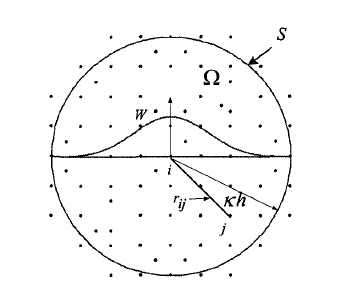
\includegraphics[scale=.8]{./images/ParticleApprox.png}
\caption{Particle approximation using particles within the support domain od the smoothing function $W$ for particle $i$. The support domain is circular with a radius of $kh$. Image 2.3 in reference \cite{Liu_SPH}}
\label{ParticleApprox}
\end{figure}
\\\textbf{Concluding remarks}\\
The computational frame in SPH are the moving particles in space.\\
The particle approximation in the SPH method is performed at every time step with particles in the current support domain, and it is done for the governing PDEs in Lagrangian description.\\
The spetial remakrs are:
\begin{enumerate}
\item The SPH method employs particles to represent the materia and form the computational frame. There is no need for predefined connectivity between these particles, all one needs is the initial particle distribution.
\item The SPH approxiamtion consists of kernel pporximation and particle approxiamtion. The kernel approxiamtion of a function and its derivative are carried out in the continuum domain, and the particle approximation of a function and its derivative are carried out using discretized particles in the support domain at the curent time step.
\item Each particle in the SPH method is associated with a support domain and influence domain.
\end{enumerate}

\section{Construction of Smoothing functions}
A smoothing function si requiered to accomplish the following properties:
\begin{enumerate}
\item The smoothing function must be normalized (\textit{Unity}) over its suport domain.
\[\int_{\Omega}{W(x-x',h)dx'}=1\]
\item The smoothing function must should be compactly supported (\textit{Compact Support})
\[W(x-x')=0,for|x-x'|>kh\]
The dimension of the compact support is defined by the smoothing function length $h$ and a scaling factor $k$, where $h$ is the smoothing length, and $k$ determines the spread of the specified smoothing function.
\item $W(x-x')\geq0$ for any point at $x'$ within the support domain of the particle at point $x$ (\textit{Positivity}) This property ensure a physically meaningful representation.
\item The smoothing function value for a aprticle should be monotonically decreasing with the increse of the distance away from the particle (\textit{Decay})
\item The smoothing function should satisfy the Dirac delta function condition
\[\lim_{h\to0}{W(x-x',h)}=\delta(x-x')\]
\item Even function
\item Smoothinf function should be sufficiently smooth
\end{enumerate}

An example of a smoothing function is the Jhonson kernel. 
\begin{figure}[h!]
\centering
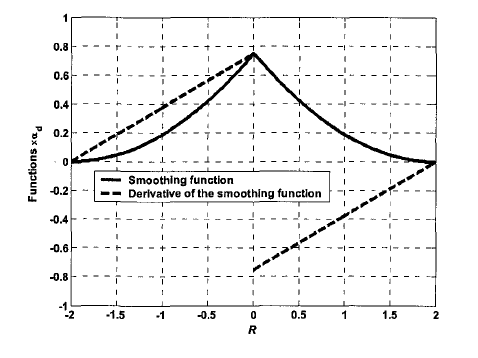
\includegraphics[scale=.8]{./images/JohnsonKernel.png}
\caption{The quadratic smoothing function and its first derivative used by Jhonson et al. (1996b). $alpha_d$ is $1/h$, $2/h$ and $5/4\pi h^3$ in one-, tow- and three-dimnesional space, respectively. Image from reference \cite{Liu_SPH}}
\label{JohnsonKernel}
\end{figure}

\section{SPH for general dynamic Fluid Flows}


\chapter{Luna}
\section{Introduction}
Fragil materials used as armour present a failure by Spalling, it is the fragil fragmentation of the material when it is being perforated. The sparced fragments are dangerous because of its high velocity.\\ \\

\textbf{Constitutive Model of Material}\\
WHen adapting the SPH formulation to solid mechanics, the strss tensor have to include the effect of the deviatoric stress. The stress tensor has two parts:
\begin{itemize}
\item Hidrostatic Pressure
\item Deviatoric Stress
\end{itemize}
\[\sigma^{\alpha\beta}=-P\delta^{\alpha\beta}+\tau^{\alpha\beta}\]
The deviatoric stress are defined with small displacements
\[\tau^{\dot{\alpha}\beta}=G\left(\epsilon^{\alpha\beta}-\frac{1}{3}\delta^{\alpha\beta}\epsilon^{\gamma\gamma}\right)\]
\begin{itemize}
\item $G$ is the shear modulus
\item $\tau^{\alpha\beta}$ is the constant stress rate
\item $\epsilon^{\alpha\beta}$ is the deformation tensor
\end{itemize}
Jaumann constitutive equation is used to descrive the deviatoric stress in a the reference system of the material:
\[\tau^{\dot{\alpha}\beta}=G\left(\epsilon^{\alpha\beta}-\frac{1}{3}\delta^{\alpha\beta}\epsilon^{\gamma\gamma}\right)+\tau^{\alpha\beta}R^{\beta\gamma}+\tau^{\alpha\beta}R^{\alpha\gamma}\]
$R$ is the rotation tensor, where rotation and deformation are defined as:
\[\epsilon^{\alpha\beta}=\frac{1}{2}\left(\frac{\partial v^\alpha}{\partial x^\beta}+\frac{\partial v^\beta}{\partial x^\alpha}\right)\]
\[R^{\alpha\beta}=\frac{1}{2}\left(\frac{\partial v^\alpha}{\partial x^\beta}-\frac{\partial v^\beta}{\partial x^\alpha}\right)\]
\\ \\
\textbf{State equation}\\
One needs to calculat pressure from the other state variables, here the Mie-Gruniensen equation is used:
\[P(e,\rho)=\left(1-\frac{1}{2}\Gamma\eta\right)P_H(\rho)+\Gamma\rho e\]
where sub-index $H$ referes to Huggoniot curve, $\Gamma$ is the Grunienesen parameter and $\eta$ is the density change rate $\eta=\frac{\rho}{\rho_0}-1$
\\ \\
\textbf{Material Model}\\ 
Luna employs the Grady\& Kipp fracture model. This model determines a statistical failures dsitribution inside the material. In SPH we need to explicity determine those failures inside the material.

\bibliography{mybib}
\bibliographystyle{unsrt}
\end{document}\